% vim: set fecn=utf8 ft=latex encoding=utf8
% -*- mode: latex; coding: UTF-8; -*-

\newif\ifdraft
\drafttrue

%%% blobtree.tex

\ifdraft
	\documentclass[conference]{acmsiggraph}
	\def\baselinestrech{1}
	\setlength{\marginparwidth}{2cm}
	\newcommand{\Title}{Implementing the Blob Tree | Draft}
\else
	\documentclass[conference]{acmsiggraph}
	\newcommand{\Title}{Implementing the Blob Tree}
\fi

\newcommand{\Author}{Evan T. C. Wilde}
\newcommand{\Email}{etcwilde@uvic.ca}
\newcommand{\Subject}{Implementing the Blob Tree}
\newcommand{\Keywords}{implicit surface, iso-surface, blobs, blobbies, blobtree}

\synctex=1

\usepackage{xspace}
\usepackage{amssymb}
\usepackage{amsmath}
\usepackage{svg}

\hypersetup{pdftitle={\Title},
        pdfauthor={\Author},
        pdfkeywords={\Keywords},
        pdfsubject={\Subject},
        urlcolor=blue,citecolor=black}

\def\BibTeX{{\rm B\kern-.05em{\sc i\kern-.025em b}\kern-.08em
    T\kern-.1667em\lower.7ex\hbox{E}\kern-.125emX}}

\TOGonlineid{000000000}
\TOGvolume{0}
\TOGnumber{0}

\ifdraft
	\usepackage[colorinlistoftodos]{todonotes}
		\newcommand{\evan}[1]{{\color{cyan}\emph{Evan Says:
		#1}}\xspace}
		\newcommand{\evanTodo}[1]{{\color{blue}\emph{Evan Todo:
		#1}}\xspace}
\else
	\usepackage[disable]{todonotes}
	\newcommand{\evan}[1]{}
	\newcommand{\evanTodo}[1]{}
\fi

\newcommand{\fff}{field falloff function}


%%% Local Variables:
%%% mode: latex
%%% TeX-master: "marching-triangles"
%%% End:


\title{\Title}
\author{
	\Author \\
	University of Victoria\\
\Email}
\pdfauthor{\Author}
\keywords{\Keywords}

\begin{document}

\teaser{
	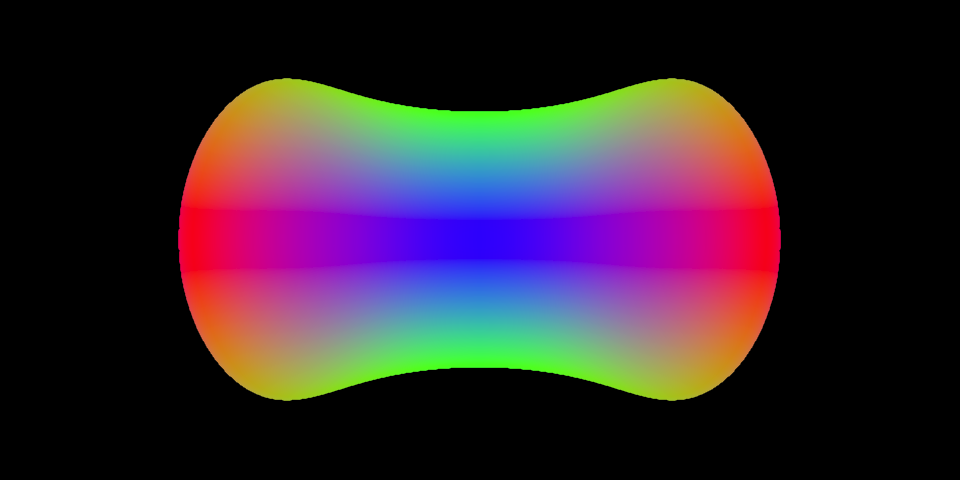
\includegraphics[height=1.5in] {images/blend.png}
	\caption{Blended Blobs}
}

\maketitle

\begin{abstract}
	Implicit surfaces are a mathematical representation of geometric
	information; storing complex geometric information with minimal memory
	requirements. Blobs are a form of implicit object defined by a central
	origin point, a \fff, and an iso value. The surface is defined at
	radius $r$ when the \fff evaluated on $r$ is equal to the iso value.

	A blob tree is used to build complex geometry from simpler
	primitives. Intelligent construction of the blob-tree is critical for
	fast evaluation of the implicit object represented in the tree, whether
	that be for ray-tracing or polygonization.

\end{abstract}

\keywordlist

\copyrightspace

\section{Introduction}
Blob trees are a data-structure for containing and evaluating the geometric
information stored by blobs.
\section{Related Work}
\section{Implementation Details}
\subsection{Transforms}
\subsection{Operations}
\subsubsection{Blend}
\subsubsection{Union}
\subsubsection{Intersect}
\subsection{Instancing}
\subsection{Normal Data}
Normal is defined by the normalized weighted linear combination of the normal
vectors of the contributing component spheres, where the weights are defined by
the contribution to the iso value of the corresponding component
sphere\cite{Wyvill}.
\subsection{Curvature}
We are looking for the principal curvatures at a given point on the surface.
The principal curvatures $k1$ and $k2$, define the curvature along the tangent
and bi-normal vectors to the given point.
Given a point $p \in \mathbb{R}^3$. Magic with matrices
happens\cite{DeAraujo2004}.
\subsection{Bounding Volume Hierarchies}
Axis-aligned bounding-boxes (AABB).

\bibliographystyle{acmsiggraph}
\bibliography{references}
\end{document}

